\documentclass[11pt, oneside]{article}   	% use "amsart" instead of "article" for AMSLaTeX format
\usepackage{geometry}                		% See geometry.pdf to learn the layout options. There are lots.
\geometry{letterpaper}                   		% ... or a4paper or a5paper or ... 
%\geometry{landscape}                		% Activate for for rotated page geometry
%\usepackage[parfill]{parskip}    		% Activate to begin paragraphs with an empty line rather than an indent
\usepackage{graphicx}				% Use pdf, png, jpg, or eps§ with pdflatex; use eps in DVI mode
								% TeX will automatically convert eps --> pdf in pdflatex		
\usepackage{amssymb}
\usepackage{amsmath}
\usepackage{parskip}
\usepackage{color}
\usepackage{hyperref}

\title{Complex function theory}
%\author{The Author}
%\section{}
%\subsection*{}
\date{}							% Activate to display a given date or no date

\graphicspath{{/Users/telliott_admin/Dropbox/Tex/png/}}
% \begin{center} 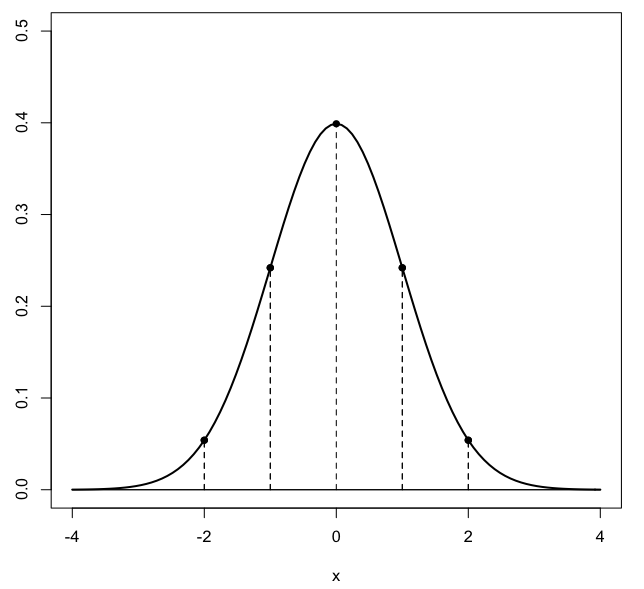
\includegraphics [scale=0.4] {gauss3.png} \end{center}
\begin{document}
\maketitle
\Large
One motivation for learning about complex functions is that the theory is often described as being very beautiful.  It also shows how certain more difficult integrals can be solved. Marsden gives three examples that he says are either very difficult or impossible if we are restricted to just the real numbers:

\[ \int_0^{\infty} \frac{\sin^2 x}{x^2} \ dx = \frac{\pi}{2} \]
\[ \int_0^{\infty} \frac{x^{\alpha - 1}}{1 + x} \ dx = \frac{\pi}{\sin \alpha \pi} \]
\[ \int_0^{2 \pi} \frac{1}{a + \sin \theta} \ d \theta = \frac{2 \pi}{\sqrt{a^2 - 1}} \]

Maybe we can learn to solve these before we're done.


\end{document} 